\section {The Arduino implementation of SOS protocol}
\begin{frame} {Outline}
    \tableofcontents [current]
\end{frame}

\begin{frame}[containsverbatim]{SOS usage}
	\begin{columns}[c]
		\begin{column}[c]{.6\textwidth}
\begin{Verbatim}[fontsize=\scriptsize]
void setup() 
{
  sos = new Sos(mac_addr, 169);
  sos->register_resource(
    resource_name, resource_name_len, 
    resource_title, resource_title_len,
    resource_rt, resource_rt_len,
    resource_handler);
}
\end{Verbatim}
		\end{column}
		\begin{column}[c]{.4\textwidth}
\begin{Verbatim}[fontsize=\scriptsize]
void loop() 
{
  sos->loop();
}
\end{Verbatim}
		\end{column}
	\end{columns}
\end{frame}

\begin{frame}[containsverbatim]{resistor and led}
	\begin{columns}[c,onlytextwidth]
		\begin{column}[c]{.5\textwidth}
			\begin{center}
				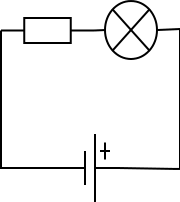
\includegraphics [width=.9\textwidth,keepaspectratio]{img/resistor_led.png}
			\end{center}
		\end{column}
		\begin{column}[c]{.5\textwidth}
\begin{Verbatim}[fontsize=\scriptsize]
uint8_t process_led(Message &in, 
	               Message &out) 
{
  int n;
  char * payload = (char*) 
    in.get_payload();
  if(payload != NULL && 
      sscanf ((const char *) payload, 
	  "val=%d", &n) == 1)
  	analogWrite(led, n);
  out.set_code(COAP_RETURN_CODE(2,5));
  return 0;
}
\end{Verbatim}
		\end{column}
	\end{columns}
\end{frame}

\begin{frame}[containsverbatim]{resistor and photoresistor}
	\begin{columns}[c,onlytextwidth]
		\begin{column}[c]{.5\textwidth}
			\begin{center}
				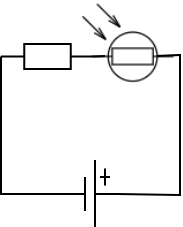
\includegraphics [width=.9\textwidth,keepaspectratio]{img/resistor_photoresistor.png}
			\end{center}
		\end{column}
		\begin{column}[c]{.5\textwidth}
\begin{Verbatim}[fontsize=\scriptsize]
uint8_t process_light(Message &in, 
                     Message &out) 
{
  char message[10];
  for(int i(0) ; i < 10 ; i++)
    message[i] = '\0';
  int sensorValue = 
    analogRead(light_sensor);
  snprintf(message, 10, "%d\0", 
                  sensorValue);
  out.set_payload( strlen(message), 
        (unsigned char *) message);
  out.set_code(COAP_RETURN_CODE(2,5));
  return 0;
}
\end{Verbatim}
		\end{column}
	\end{columns}
\end{frame}

\begin{frame}[containsverbatim]{Thermistor}
	\begin{columns}[c,onlytextwidth]
		\begin{column}[c]{.5\textwidth}
			\begin{center}
				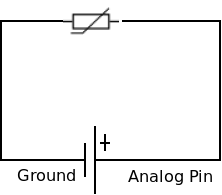
\includegraphics [width=.9\textwidth,keepaspectratio]{img/thermistor.png}
			\end{center}
		\end{column}
		\begin{column}[c]{.5\textwidth}
\begin{Verbatim}[fontsize=\scriptsize]
uint8_t temperature_handler(Message &in, 
                           Message &out) 
{
  char message[10];
  for(int i(0) ; i < 10 ; i++)
    message[i] = '\0';
  int sensorValue = 
    analogRead(tmp_sensor);
  snprintf(message, 10, "%d\0", 
                  sensorValue);
  out.set_payload( strlen(message), 
        (unsigned char *) message);
  out.set_code(COAP_RETURN_CODE(2,5));
  return 0;
}
\end{Verbatim}
		\end{column}
	\end{columns}
\end{frame}

\begin{frame} {Difficulties}
    \begin{itemize}
		\item SRAM = 2Ko
		\item W5100 : easy in UDP and TCP mode, less in MAC Raw
		\item no debug facility
		\begin{itemize}
			\item no gdb, no valgrind
			\item when the program reboots : no warning message
		\end{itemize}
		\item packet loss on busy network
    \end{itemize}
\end{frame}


